\section*{Diseño de Algoritmos y Diagramas de Flujo}

Los diagramas de flujo son soluciones entendibles en lenguaje humano para determinado problema. Es una representación visual de un Algoritmo.

Los elementos que poseen los diagramas de flujo son los siguientes:
\begin{center}
    \begin{tabular}{ c c  }
        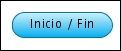
\includegraphics[scale=1.3]{Imagenes/image04} & 
        Inicio o fin  \\ 
        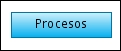
\includegraphics[scale=1.3]{Imagenes/image07} & Pasos, procesos o líneas de instrucción del programa.  \\  
        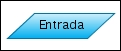
\includegraphics[scale=1.3]{Imagenes/image00} & Operaciones de entrada o salida ("pedir" o "mostrar/escribir" datos).  \\  
        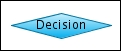
\includegraphics[scale=1.3]{Imagenes/image09} & Toma de decisiones, elecciones y ramificaciones.
    \end{tabular}
\end{center}

\section*{Ejercicios}
\begin{itemize}
    \item Identificar\\
        ¿Que hacen los siguientes diagramas de flujo?
          \begin{center}
            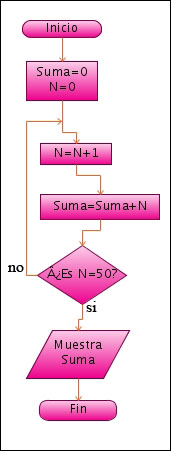
\includegraphics[scale=0.5]{Imagenes/image11}.
            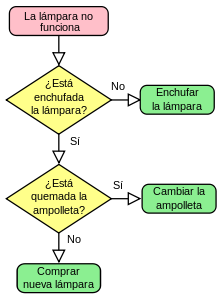
\includegraphics[scale=0.8]{Imagenes/image03}
          \end{center}

    \item Muchos ejercicios\\
        \begin{enumerate}
            \item Haga un diagrama de flujo que determine si el número entero ingresado por el usuario es par o no.
            \item Haga un diagrama de flujo que imprima los números impares entre 1 y 200.
            \item Haga un diagrama de flujo que pida al usuario un número N, y luego responda si aquel número es primo o no.
            \item Pitágoras en conjunto con Boole, L’hopital y Laplace necesitan un programa que pueda generar los números primos menores de 300. Haga un diagrama de flujo  que haga esto y los muestre por pantalla.
            \item Haga un diagrama de flujo  que reciba un número N y retorne el factorial de este. Recuerde que el factorial de N se denota N! y es igual a 1*2*3*4*...*N.
            \item Haga un diagrama de flujo que reciba 2 números enteros, y entregue el resultado de la división entera entre estos, indicando si la división entre ellos es exacta o no.
            \item Haga un diagrama de flujo que reciba 2 palabras y que indique cual de ellas es la más larga, y por cuanto lo es.
            \item Haga un diagrama de flujo muestre la tabla de multiplicación desde el número 1 hasta el número 10 de un número N ingresado por el usuario.
        \end{enumerate}
\end{itemize}
